\documentclass[twoside]{book}

% Packages required by doxygen
\usepackage{fixltx2e}
\usepackage{calc}
\usepackage{doxygen}
\usepackage[export]{adjustbox} % also loads graphicx
\usepackage{graphicx}
\usepackage[utf8]{inputenc}
\usepackage{makeidx}
\usepackage{multicol}
\usepackage{multirow}
\PassOptionsToPackage{warn}{textcomp}
\usepackage{textcomp}
\usepackage[nointegrals]{wasysym}
\usepackage[table]{xcolor}

% Font selection
\usepackage[T1]{fontenc}
\usepackage[scaled=.90]{helvet}
\usepackage{courier}
\usepackage{amssymb}
\usepackage{sectsty}
\renewcommand{\familydefault}{\sfdefault}
\allsectionsfont{%
  \fontseries{bc}\selectfont%
  \color{darkgray}%
}
\renewcommand{\DoxyLabelFont}{%
  \fontseries{bc}\selectfont%
  \color{darkgray}%
}
\newcommand{\+}{\discretionary{\mbox{\scriptsize$\hookleftarrow$}}{}{}}

% Page & text layout
\usepackage{geometry}
\geometry{%
  a4paper,%
  top=2.5cm,%
  bottom=2.5cm,%
  left=2.5cm,%
  right=2.5cm%
}
\tolerance=750
\hfuzz=15pt
\hbadness=750
\setlength{\emergencystretch}{15pt}
\setlength{\parindent}{0cm}
\setlength{\parskip}{3ex plus 2ex minus 2ex}
\makeatletter
\renewcommand{\paragraph}{%
  \@startsection{paragraph}{4}{0ex}{-1.0ex}{1.0ex}{%
    \normalfont\normalsize\bfseries\SS@parafont%
  }%
}
\renewcommand{\subparagraph}{%
  \@startsection{subparagraph}{5}{0ex}{-1.0ex}{1.0ex}{%
    \normalfont\normalsize\bfseries\SS@subparafont%
  }%
}
\makeatother

% Headers & footers
\usepackage{fancyhdr}
\pagestyle{fancyplain}
\fancyhead[LE]{\fancyplain{}{\bfseries\thepage}}
\fancyhead[CE]{\fancyplain{}{}}
\fancyhead[RE]{\fancyplain{}{\bfseries\leftmark}}
\fancyhead[LO]{\fancyplain{}{\bfseries\rightmark}}
\fancyhead[CO]{\fancyplain{}{}}
\fancyhead[RO]{\fancyplain{}{\bfseries\thepage}}
\fancyfoot[LE]{\fancyplain{}{}}
\fancyfoot[CE]{\fancyplain{}{}}
\fancyfoot[RE]{\fancyplain{}{\bfseries\scriptsize Generated by Doxygen }}
\fancyfoot[LO]{\fancyplain{}{\bfseries\scriptsize Generated by Doxygen }}
\fancyfoot[CO]{\fancyplain{}{}}
\fancyfoot[RO]{\fancyplain{}{}}
\renewcommand{\footrulewidth}{0.4pt}
\renewcommand{\chaptermark}[1]{%
  \markboth{#1}{}%
}
\renewcommand{\sectionmark}[1]{%
  \markright{\thesection\ #1}%
}

% Indices & bibliography
\usepackage{natbib}
\usepackage[titles]{tocloft}
\setcounter{tocdepth}{3}
\setcounter{secnumdepth}{5}
\makeindex

% Hyperlinks (required, but should be loaded last)
\usepackage{ifpdf}
\ifpdf
  \usepackage[pdftex,pagebackref=true]{hyperref}
\else
  \usepackage[ps2pdf,pagebackref=true]{hyperref}
\fi
\hypersetup{%
  colorlinks=true,%
  linkcolor=blue,%
  citecolor=blue,%
  unicode%
}

% Custom commands
\newcommand{\clearemptydoublepage}{%
  \newpage{\pagestyle{empty}\cleardoublepage}%
}

\usepackage{caption}
\captionsetup{labelsep=space,justification=centering,font={bf},singlelinecheck=off,skip=4pt,position=top}

%===== C O N T E N T S =====

\begin{document}

% Titlepage & ToC
\hypersetup{pageanchor=false,
             bookmarksnumbered=true,
             pdfencoding=unicode
            }
\pagenumbering{alph}
\begin{titlepage}
\vspace*{7cm}
\begin{center}%
{\Large Projet moyenne }\\
\vspace*{1cm}
{\large Generated by Doxygen 1.8.13}\\
\end{center}
\end{titlepage}
\clearemptydoublepage
\pagenumbering{roman}
\tableofcontents
\clearemptydoublepage
\pagenumbering{arabic}
\hypersetup{pageanchor=true}

%--- Begin generated contents ---
\chapter{Namespace Index}
\section{Packages}
Here are the packages with brief descriptions (if available)\+:\begin{DoxyCompactList}
\item\contentsline{section}{\hyperlink{namespace_moyenne}{Moyenne} }{\pageref{namespace_moyenne}}{}
\item\contentsline{section}{\hyperlink{namespace_moyenne_1_1_properties}{Moyenne.\+Properties} }{\pageref{namespace_moyenne_1_1_properties}}{}
\end{DoxyCompactList}

\chapter{Hierarchical Index}
\section{Class Hierarchy}
This inheritance list is sorted roughly, but not completely, alphabetically\+:\begin{DoxyCompactList}
\item \contentsline{section}{Moyenne.\+Connection\+DB}{\pageref{class_moyenne_1_1_connection_d_b}}{}
\item \contentsline{section}{Moyenne.\+Eleve}{\pageref{class_moyenne_1_1_eleve}}{}
\item Form\begin{DoxyCompactList}
\item \contentsline{section}{Moyenne.\+frm\+Classe}{\pageref{class_moyenne_1_1frm_classe}}{}
\item \contentsline{section}{Moyenne.\+frm\+Eleve}{\pageref{class_moyenne_1_1frm_eleve}}{}
\item \contentsline{section}{Moyenne.\+frm\+Saisie\+Note}{\pageref{class_moyenne_1_1frm_saisie_note}}{}
\end{DoxyCompactList}
\item \contentsline{section}{Moyenne.\+Note}{\pageref{class_moyenne_1_1_note}}{}
\end{DoxyCompactList}

\chapter{Class Index}
\section{Class List}
Here are the classes, structs, unions and interfaces with brief descriptions\+:\begin{DoxyCompactList}
\item\contentsline{section}{\hyperlink{class_moyenne_1_1_connection_d_b}{Moyenne.\+Connection\+DB} }{\pageref{class_moyenne_1_1_connection_d_b}}{}
\item\contentsline{section}{\hyperlink{class_moyenne_1_1_eleve}{Moyenne.\+Eleve} }{\pageref{class_moyenne_1_1_eleve}}{}
\item\contentsline{section}{\hyperlink{class_moyenne_1_1frm_classe}{Moyenne.\+frm\+Classe} }{\pageref{class_moyenne_1_1frm_classe}}{}
\item\contentsline{section}{\hyperlink{class_moyenne_1_1frm_eleve}{Moyenne.\+frm\+Eleve} }{\pageref{class_moyenne_1_1frm_eleve}}{}
\item\contentsline{section}{\hyperlink{class_moyenne_1_1frm_saisie_note}{Moyenne.\+frm\+Saisie\+Note} }{\pageref{class_moyenne_1_1frm_saisie_note}}{}
\item\contentsline{section}{\hyperlink{class_moyenne_1_1_note}{Moyenne.\+Note} }{\pageref{class_moyenne_1_1_note}}{}
\end{DoxyCompactList}

\chapter{Namespace Documentation}
\hypertarget{namespace_moyenne}{}\section{Moyenne Namespace Reference}
\label{namespace_moyenne}\index{Moyenne@{Moyenne}}
\subsection*{Namespaces}
\begin{DoxyCompactItemize}
\end{DoxyCompactItemize}
\subsection*{Classes}
\begin{DoxyCompactItemize}
\item 
class \hyperlink{class_moyenne_1_1_connection_d_b}{Connection\+DB}
\item 
class \hyperlink{class_moyenne_1_1_eleve}{Eleve}
\item 
class \hyperlink{class_moyenne_1_1frm_classe}{frm\+Classe}
\item 
class \hyperlink{class_moyenne_1_1frm_eleve}{frm\+Eleve}
\item 
class \hyperlink{class_moyenne_1_1frm_saisie_note}{frm\+Saisie\+Note}
\item 
class \hyperlink{class_moyenne_1_1_note}{Note}
\item 
class {\bfseries Program}
\end{DoxyCompactItemize}

\hypertarget{namespace_moyenne_1_1_properties}{}\section{Moyenne.\+Properties Namespace Reference}
\label{namespace_moyenne_1_1_properties}\index{Moyenne.\+Properties@{Moyenne.\+Properties}}
\subsection*{Classes}
\begin{DoxyCompactItemize}
\item 
class {\bfseries Resources}
\begin{DoxyCompactList}\small\item\em A strongly-\/typed resource class, for looking up localized strings, etc. \end{DoxyCompactList}\item 
class {\bfseries Settings}
\end{DoxyCompactItemize}

\chapter{Class Documentation}
\hypertarget{class_moyenne_1_1_connection_d_b}{}\section{Moyenne.\+Connection\+DB Class Reference}
\label{class_moyenne_1_1_connection_d_b}\index{Moyenne.\+Connection\+DB@{Moyenne.\+Connection\+DB}}
\subsection*{Public Member Functions}
\begin{DoxyCompactItemize}
\item 
\mbox{\Hypertarget{class_moyenne_1_1_connection_d_b_a22de5667092474c01745891870e1f0ec}\label{class_moyenne_1_1_connection_d_b_a22de5667092474c01745891870e1f0ec}} 
void {\bfseries Add\+Eleve} (\hyperlink{class_moyenne_1_1_eleve}{Eleve} eleve)
\item 
\mbox{\Hypertarget{class_moyenne_1_1_connection_d_b_a6ef1b54a6f7a45e6c11b487032dea1fa}\label{class_moyenne_1_1_connection_d_b_a6ef1b54a6f7a45e6c11b487032dea1fa}} 
List$<$ \hyperlink{class_moyenne_1_1_eleve}{Eleve} $>$ {\bfseries get\+Eleves} ()
\end{DoxyCompactItemize}


The documentation for this class was generated from the following file\+:\begin{DoxyCompactItemize}
\item 
Moyenne/Connection\+D\+B.\+cs\end{DoxyCompactItemize}

\hypertarget{class_moyenne_1_1_eleve}{}\section{Moyenne.\+Eleve Class Reference}
\label{class_moyenne_1_1_eleve}\index{Moyenne.\+Eleve@{Moyenne.\+Eleve}}
\subsection*{Public Member Functions}
\begin{DoxyCompactItemize}
\item 
\mbox{\Hypertarget{class_moyenne_1_1_eleve_a0004c2843368a1bbf9ce62778a49379a}\label{class_moyenne_1_1_eleve_a0004c2843368a1bbf9ce62778a49379a}} 
override string {\bfseries To\+String} ()
\end{DoxyCompactItemize}
\subsection*{Properties}
\begin{DoxyCompactItemize}
\item 
\mbox{\Hypertarget{class_moyenne_1_1_eleve_a3ebbcd846ecb67e09f70d9955a458dce}\label{class_moyenne_1_1_eleve_a3ebbcd846ecb67e09f70d9955a458dce}} 
string {\bfseries Nom}\hspace{0.3cm}{\ttfamily  \mbox{[}get, set\mbox{]}}
\item 
\mbox{\Hypertarget{class_moyenne_1_1_eleve_aeef8953ec6c139263caa9acfe8ffa11c}\label{class_moyenne_1_1_eleve_aeef8953ec6c139263caa9acfe8ffa11c}} 
string {\bfseries Prenom}\hspace{0.3cm}{\ttfamily  \mbox{[}get, set\mbox{]}}
\item 
\mbox{\Hypertarget{class_moyenne_1_1_eleve_af6878eddddb9eb7247c0ddd6e49fd740}\label{class_moyenne_1_1_eleve_af6878eddddb9eb7247c0ddd6e49fd740}} 
float {\bfseries Moyenne}\hspace{0.3cm}{\ttfamily  \mbox{[}get, set\mbox{]}}
\item 
\mbox{\Hypertarget{class_moyenne_1_1_eleve_a38b165e62ba0ac45fe692a1cb2c94c02}\label{class_moyenne_1_1_eleve_a38b165e62ba0ac45fe692a1cb2c94c02}} 
List$<$ \hyperlink{class_moyenne_1_1_note}{Note} $>$ {\bfseries Lst\+Notes}\hspace{0.3cm}{\ttfamily  \mbox{[}get, set\mbox{]}}
\end{DoxyCompactItemize}


The documentation for this class was generated from the following file\+:\begin{DoxyCompactItemize}
\item 
Moyenne/Eleve.\+cs\end{DoxyCompactItemize}

\hypertarget{class_moyenne_1_1frm_classe}{}\section{Moyenne.\+frm\+Classe Class Reference}
\label{class_moyenne_1_1frm_classe}\index{Moyenne.\+frm\+Classe@{Moyenne.\+frm\+Classe}}
Inheritance diagram for Moyenne.\+frm\+Classe\+:\begin{figure}[H]
\begin{center}
\leavevmode
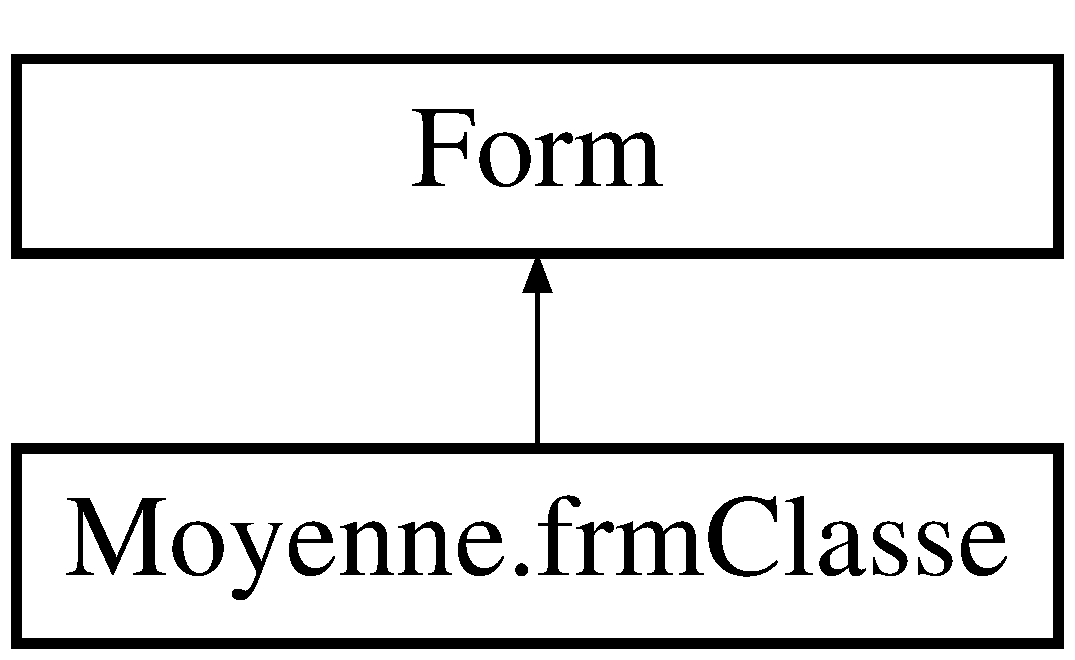
\includegraphics[height=2.000000cm]{class_moyenne_1_1frm_classe}
\end{center}
\end{figure}
\subsection*{Protected Member Functions}
\begin{DoxyCompactItemize}
\item 
override void \hyperlink{class_moyenne_1_1frm_classe_ae7baf72f6e4d6fb0f6ad3e65b9a6c580}{Dispose} (bool disposing)
\begin{DoxyCompactList}\small\item\em Clean up any resources being used. \end{DoxyCompactList}\end{DoxyCompactItemize}


\subsection{Member Function Documentation}
\mbox{\Hypertarget{class_moyenne_1_1frm_classe_ae7baf72f6e4d6fb0f6ad3e65b9a6c580}\label{class_moyenne_1_1frm_classe_ae7baf72f6e4d6fb0f6ad3e65b9a6c580}} 
\index{Moyenne\+::frm\+Classe@{Moyenne\+::frm\+Classe}!Dispose@{Dispose}}
\index{Dispose@{Dispose}!Moyenne\+::frm\+Classe@{Moyenne\+::frm\+Classe}}
\subsubsection{\texorpdfstring{Dispose()}{Dispose()}}
{\footnotesize\ttfamily override void Moyenne.\+frm\+Classe.\+Dispose (\begin{DoxyParamCaption}\item[{bool}]{disposing }\end{DoxyParamCaption})\hspace{0.3cm}{\ttfamily [protected]}}



Clean up any resources being used. 


\begin{DoxyParams}{Parameters}
{\em disposing} & true if managed resources should be disposed; otherwise, false.\\
\hline
\end{DoxyParams}


The documentation for this class was generated from the following files\+:\begin{DoxyCompactItemize}
\item 
Moyenne/frm\+Classe.\+cs\item 
Moyenne/frm\+Classe.\+Designer.\+cs\end{DoxyCompactItemize}

\hypertarget{class_moyenne_1_1frm_eleve}{}\section{Moyenne.\+frm\+Eleve Class Reference}
\label{class_moyenne_1_1frm_eleve}\index{Moyenne.\+frm\+Eleve@{Moyenne.\+frm\+Eleve}}
Inheritance diagram for Moyenne.\+frm\+Eleve\+:\begin{figure}[H]
\begin{center}
\leavevmode
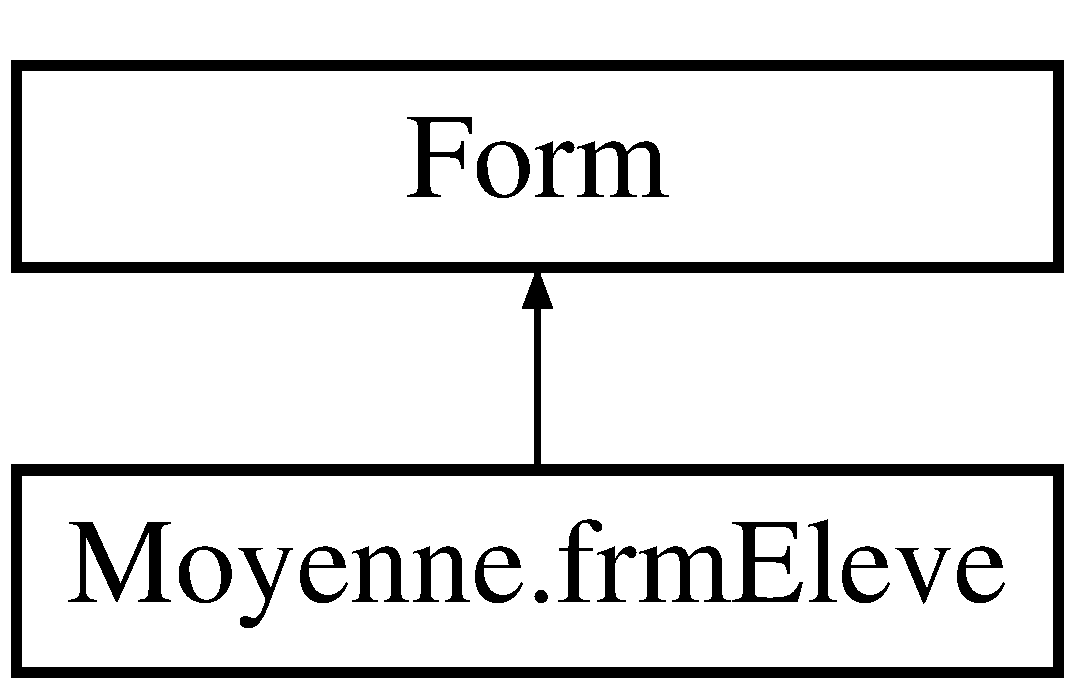
\includegraphics[height=2.000000cm]{class_moyenne_1_1frm_eleve}
\end{center}
\end{figure}
\subsection*{Public Attributes}
\begin{DoxyCompactItemize}
\item 
\mbox{\Hypertarget{class_moyenne_1_1frm_eleve_a96e485d73fdd41f75e323888627e4cc1}\label{class_moyenne_1_1frm_eleve_a96e485d73fdd41f75e323888627e4cc1}} 
\hyperlink{class_moyenne_1_1_eleve}{Eleve} {\bfseries eleve}
\item 
\mbox{\Hypertarget{class_moyenne_1_1frm_eleve_a566d185b38c1066b802d71d323d33b81}\label{class_moyenne_1_1frm_eleve_a566d185b38c1066b802d71d323d33b81}} 
System.\+Windows.\+Forms.\+Text\+Box {\bfseries txt\+Nom}
\item 
\mbox{\Hypertarget{class_moyenne_1_1frm_eleve_a6bc0c3da466fcad44a803b0a879a8775}\label{class_moyenne_1_1frm_eleve_a6bc0c3da466fcad44a803b0a879a8775}} 
System.\+Windows.\+Forms.\+Text\+Box {\bfseries txt\+Prenom}
\item 
\mbox{\Hypertarget{class_moyenne_1_1frm_eleve_aff501043537d2300e18e2fd030add04a}\label{class_moyenne_1_1frm_eleve_aff501043537d2300e18e2fd030add04a}} 
System.\+Windows.\+Forms.\+Label {\bfseries lbl\+Res\+Moyenne}
\end{DoxyCompactItemize}
\subsection*{Protected Member Functions}
\begin{DoxyCompactItemize}
\item 
override void \hyperlink{class_moyenne_1_1frm_eleve_a4cd27dbd3a275339051774b7faf22331}{Dispose} (bool disposing)
\begin{DoxyCompactList}\small\item\em Clean up any resources being used. \end{DoxyCompactList}\end{DoxyCompactItemize}


\subsection{Member Function Documentation}
\mbox{\Hypertarget{class_moyenne_1_1frm_eleve_a4cd27dbd3a275339051774b7faf22331}\label{class_moyenne_1_1frm_eleve_a4cd27dbd3a275339051774b7faf22331}} 
\index{Moyenne\+::frm\+Eleve@{Moyenne\+::frm\+Eleve}!Dispose@{Dispose}}
\index{Dispose@{Dispose}!Moyenne\+::frm\+Eleve@{Moyenne\+::frm\+Eleve}}
\subsubsection{\texorpdfstring{Dispose()}{Dispose()}}
{\footnotesize\ttfamily override void Moyenne.\+frm\+Eleve.\+Dispose (\begin{DoxyParamCaption}\item[{bool}]{disposing }\end{DoxyParamCaption})\hspace{0.3cm}{\ttfamily [protected]}}



Clean up any resources being used. 


\begin{DoxyParams}{Parameters}
{\em disposing} & true if managed resources should be disposed; otherwise, false.\\
\hline
\end{DoxyParams}


The documentation for this class was generated from the following files\+:\begin{DoxyCompactItemize}
\item 
Moyenne/frm\+Eleve.\+cs\item 
Moyenne/frm\+Eleve.\+Designer.\+cs\end{DoxyCompactItemize}

\hypertarget{class_moyenne_1_1frm_saisie_note}{}\section{Moyenne.\+frm\+Saisie\+Note Class Reference}
\label{class_moyenne_1_1frm_saisie_note}\index{Moyenne.\+frm\+Saisie\+Note@{Moyenne.\+frm\+Saisie\+Note}}
Inheritance diagram for Moyenne.\+frm\+Saisie\+Note\+:\begin{figure}[H]
\begin{center}
\leavevmode
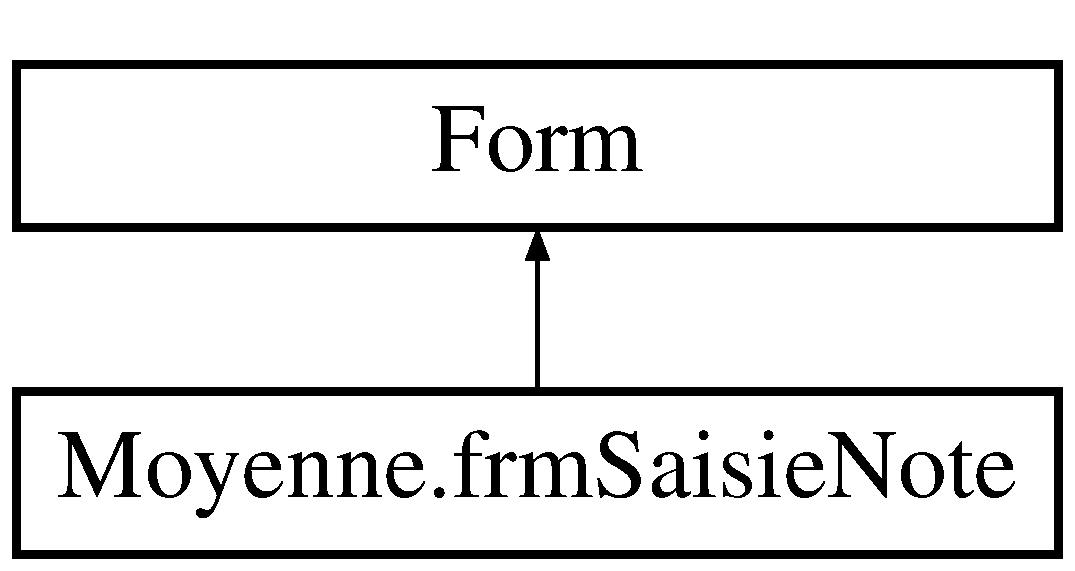
\includegraphics[height=2.000000cm]{class_moyenne_1_1frm_saisie_note}
\end{center}
\end{figure}
\subsection*{Public Attributes}
\begin{DoxyCompactItemize}
\item 
\mbox{\Hypertarget{class_moyenne_1_1frm_saisie_note_a2ae44fbf3eb13e3c2be910451a1660e2}\label{class_moyenne_1_1frm_saisie_note_a2ae44fbf3eb13e3c2be910451a1660e2}} 
\hyperlink{class_moyenne_1_1_note}{Note} {\bfseries note}
\item 
\mbox{\Hypertarget{class_moyenne_1_1frm_saisie_note_aa9943d0221bf23b31dee4c84af92583b}\label{class_moyenne_1_1frm_saisie_note_aa9943d0221bf23b31dee4c84af92583b}} 
System.\+Windows.\+Forms.\+Numeric\+Up\+Down {\bfseries nud\+Entier}
\item 
\mbox{\Hypertarget{class_moyenne_1_1frm_saisie_note_a5e7a2d1caafffe863cd6aae2c968f3b5}\label{class_moyenne_1_1frm_saisie_note_a5e7a2d1caafffe863cd6aae2c968f3b5}} 
System.\+Windows.\+Forms.\+Numeric\+Up\+Down {\bfseries nud\+Decimal}
\end{DoxyCompactItemize}
\subsection*{Protected Member Functions}
\begin{DoxyCompactItemize}
\item 
override void \hyperlink{class_moyenne_1_1frm_saisie_note_a3368c473ed5efe48547f79ebff70a0f5}{Dispose} (bool disposing)
\begin{DoxyCompactList}\small\item\em Clean up any resources being used. \end{DoxyCompactList}\end{DoxyCompactItemize}


\subsection{Member Function Documentation}
\mbox{\Hypertarget{class_moyenne_1_1frm_saisie_note_a3368c473ed5efe48547f79ebff70a0f5}\label{class_moyenne_1_1frm_saisie_note_a3368c473ed5efe48547f79ebff70a0f5}} 
\index{Moyenne\+::frm\+Saisie\+Note@{Moyenne\+::frm\+Saisie\+Note}!Dispose@{Dispose}}
\index{Dispose@{Dispose}!Moyenne\+::frm\+Saisie\+Note@{Moyenne\+::frm\+Saisie\+Note}}
\subsubsection{\texorpdfstring{Dispose()}{Dispose()}}
{\footnotesize\ttfamily override void Moyenne.\+frm\+Saisie\+Note.\+Dispose (\begin{DoxyParamCaption}\item[{bool}]{disposing }\end{DoxyParamCaption})\hspace{0.3cm}{\ttfamily [protected]}}



Clean up any resources being used. 


\begin{DoxyParams}{Parameters}
{\em disposing} & true if managed resources should be disposed; otherwise, false.\\
\hline
\end{DoxyParams}


The documentation for this class was generated from the following files\+:\begin{DoxyCompactItemize}
\item 
Moyenne/frm\+Saisie\+Note.\+cs\item 
Moyenne/frm\+Saisie\+Note.\+Designer.\+cs\end{DoxyCompactItemize}

\hypertarget{class_moyenne_1_1_note}{}\section{Moyenne.\+Note Class Reference}
\label{class_moyenne_1_1_note}\index{Moyenne.\+Note@{Moyenne.\+Note}}
\subsection*{Public Member Functions}
\begin{DoxyCompactItemize}
\item 
\mbox{\Hypertarget{class_moyenne_1_1_note_abf8d504fdae5f75270fc06073cd2e055}\label{class_moyenne_1_1_note_abf8d504fdae5f75270fc06073cd2e055}} 
{\bfseries Note} (int dizieme)
\item 
\mbox{\Hypertarget{class_moyenne_1_1_note_a988f0e03904ac78184a43c67a962849d}\label{class_moyenne_1_1_note_a988f0e03904ac78184a43c67a962849d}} 
override string {\bfseries To\+String} ()
\item 
\mbox{\Hypertarget{class_moyenne_1_1_note_acac42334c72a6006967b068e3ee371da}\label{class_moyenne_1_1_note_acac42334c72a6006967b068e3ee371da}} 
bool {\bfseries Is\+Note\+Correcte} ()
\end{DoxyCompactItemize}
\subsection*{Static Public Member Functions}
\begin{DoxyCompactItemize}
\item 
static float \hyperlink{class_moyenne_1_1_note_afcbbe7434fea2a87085b201dc07289a4}{Calcul\+Moyenne} (List\+Box liste\+Notes)
\begin{DoxyCompactList}\small\item\em Calcule moyenne de l\textquotesingle{}élève \end{DoxyCompactList}\item 
\mbox{\Hypertarget{class_moyenne_1_1_note_adb651595cf0c4b15c41d55228704f15a}\label{class_moyenne_1_1_note_adb651595cf0c4b15c41d55228704f15a}} 
static float {\bfseries Somme\+Notes} (List\+Box liste\+Notes)
\item 
\mbox{\Hypertarget{class_moyenne_1_1_note_aa8f1a8abb95aba277e4a98c29b0168c3}\label{class_moyenne_1_1_note_aa8f1a8abb95aba277e4a98c29b0168c3}} 
static List$<$ \hyperlink{class_moyenne_1_1_note}{Note} $>$ {\bfseries Get\+Liste\+Notes} (List\+Box liste\+Notes)
\end{DoxyCompactItemize}
\subsection*{Properties}
\begin{DoxyCompactItemize}
\item 
\mbox{\Hypertarget{class_moyenne_1_1_note_a911af875364929c6de36718f8330fa5b}\label{class_moyenne_1_1_note_a911af875364929c6de36718f8330fa5b}} 
int {\bfseries Valeur\+Dizieme}\hspace{0.3cm}{\ttfamily  \mbox{[}get, set\mbox{]}}
\end{DoxyCompactItemize}


\subsection{Member Function Documentation}
\mbox{\Hypertarget{class_moyenne_1_1_note_afcbbe7434fea2a87085b201dc07289a4}\label{class_moyenne_1_1_note_afcbbe7434fea2a87085b201dc07289a4}} 
\index{Moyenne\+::\+Note@{Moyenne\+::\+Note}!Calcul\+Moyenne@{Calcul\+Moyenne}}
\index{Calcul\+Moyenne@{Calcul\+Moyenne}!Moyenne\+::\+Note@{Moyenne\+::\+Note}}
\subsubsection{\texorpdfstring{Calcul\+Moyenne()}{CalculMoyenne()}}
{\footnotesize\ttfamily static float Moyenne.\+Note.\+Calcul\+Moyenne (\begin{DoxyParamCaption}\item[{List\+Box}]{liste\+Notes }\end{DoxyParamCaption})\hspace{0.3cm}{\ttfamily [static]}}



Calcule moyenne de l\textquotesingle{}élève 


\begin{DoxyParams}{Parameters}
{\em liste\+Notes} & \\
\hline
\end{DoxyParams}
\begin{DoxyReturn}{Returns}
moyenne
\end{DoxyReturn}


The documentation for this class was generated from the following file\+:\begin{DoxyCompactItemize}
\item 
Moyenne/Note.\+cs\end{DoxyCompactItemize}

%--- End generated contents ---

% Index
\backmatter
\newpage
\phantomsection
\clearemptydoublepage
\addcontentsline{toc}{chapter}{Index}
\printindex

\end{document}
